\section{Experiment Score}
\label{sec:experiment}

This section presents the experimental results validating our implementation, structured into two main parts: demonstration of iterative decoding and reporting of the best FID scores obtained.

\subsection{Iterative Decoding}
In this part, we demonstrate the iterative decoding process for different mask scheduling strategies.

\subsubsection{Mask in Latent Domain}
Present visualizations of the mask distribution over iterations using different scheduling strategies (cosine, linear, square).

\begin{figure}[H]
    \centering
    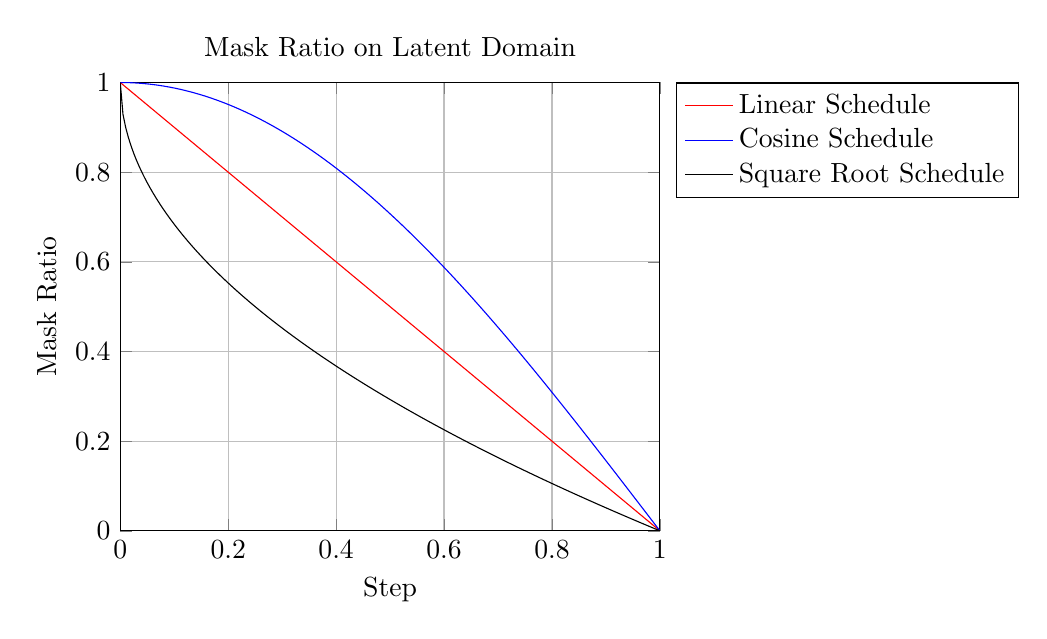
\begin{tikzpicture}
        \begin{axis}[
                % width=0.4\linewidth,
                % height=0.4\linewidth,
                grid=major,
                title={Mask Ratio on Latent Domain},
                legend pos=outer north east,
                legend cell align=left,
                xmin=0,xmax=1,
                ymin=0,ymax=1,
                xlabel={Step},
                ylabel={Mask Ratio},
            ]
            \addplot[domain=0:1,samples=200,red]{1-x};
            \addlegendentry{Linear Schedule}
            \addplot[domain=0:1,samples=200,blue]{(cos(deg(x)*pi/2))};
            \addlegendentry{Cosine Schedule}
            % \addplot[domain=0:1,samples=200,magenta]{1-x^2};
            % \addlegendentry{Square Schedule}
            \addplot[domain=0:1,samples=200,black]{(1-sqrt(x))};
            \addlegendentry{Square Root Schedule}
        \end{axis}
    \end{tikzpicture}
\end{figure}

% a figure with 3 subfigure latent figures, horrizontal stacked

\begin{figure}[H]
    \begin{minipage}[t]{0.3\textwidth}
        \centering
        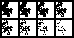
\includegraphics[width=\textwidth]{images/cosine_mask_test_0.png}
        \subcaption{Cosine Schedule}
        \label{fig:mask_latent_cosine}
    \end{minipage}%
    \hfill
    \begin{minipage}[t]{0.3\textwidth}
        \centering
        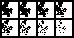
\includegraphics[width=\textwidth]{images/linear_mask_test_0.png}
        \subcaption{Linear Schedule}
        \label{fig:mask_latent_linear}
    \end{minipage}%
    \hfill
    \begin{minipage}[t]{0.3\textwidth}
        \centering
        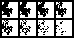
\includegraphics[width=\textwidth]{images/sqrt_mask_test_0.png}
        \subcaption{Square Root Schedule}
        \label{fig:mask_latent_sqrt}
    \end{minipage}
    \caption{Mask in Latent Domain with Different Schedules. Three of this schedule are generated with the same image.}
    \label{fig:mask_latent}
\end{figure}

\subsubsection{Predicted Images}

% Show the intermediate predicted images at different decoding iterations using the scheduling strategies.

The intermediate predicted images at different decoding iterations are shown in Figures \ref{fig:predicted_cosine}, \ref{fig:predicted_linear}, and \ref{fig:predicted_sqrt}.
The images illustrate the model's ability to progressively fill in the masked regions, demonstrating the effectiveness of the iterative decoding process.

\begin{figure}[H]
    \begin{minipage}[t]{0.3\textwidth}
        \centering
        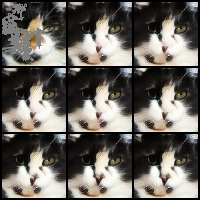
\includegraphics[width=\textwidth]{images/cosine_pred_test_0.png}
        \subcaption{Cosine Schedule}
        \label{fig:predicted_cosine}
    \end{minipage}
    \hfill
    \begin{minipage}[t]{0.3\textwidth}
        \centering
        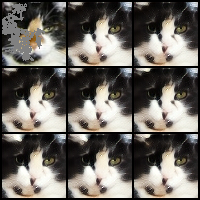
\includegraphics[width=\textwidth]{images/linear_pred_test_0.png}
        \subcaption{Linear Schedule}
        \label{fig:predicted_linear}
    \end{minipage}
    \hfill
    \begin{minipage}[t]{0.3\textwidth}
        \centering
        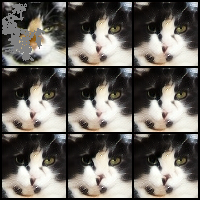
\includegraphics[width=\textwidth]{images/sqrt_pred_test_0.png}
        \subcaption{Square Root Schedule}
        \label{fig:predicted_sqrt}
    \end{minipage}
    \caption{Predicted Images at Different Iterations. The images show the model's iterative refinement process.}
    \label{fig:predicted}
\end{figure}

The predicted images for the linear schedule are shown in Figure \ref{fig:predicted_linear}. The images demonstrate the iterative refinement process, where the model progressively fills in the masked regions.

\subsection{Best FID Score}

\subsubsection{Results}

The FID scores obtained from the experiments are summarized in Table \ref{tab:fid_scores}.
The scores indicate the quality of the generated images, with lower scores indicating better performance.

\begin{table}[H]
    \centering
    \caption{FID Scores for Different Mask Scheduling Strategies}
    \label{tab:fid_scores}
    \begin{tabular}{c||c}
        \textbf{Mask Scheduling Strategy} & \textbf{FID Score} \\ \hline\hline
        Cosine Schedule                   & 38.02              \\ \hline
        Linear Schedule                   & 39.12              \\ \hline
        Square Root Schedule              & 39.30              \\ \hline
    \end{tabular}
\end{table}

\subsubsection{Experimental Settings}

The experiments were conducted with the following settings:

\begin{itemize}
    \item \textbf{Learning Rate:} $1\times10^{-4}$
    \item \textbf{Batch Size:} $32$
    \item \textbf{Epochs:} $200$
    \item \textbf{Sweet Spot:} $8$
    \item \textbf{Total Iterations:} $8$
\end{itemize}


And the results shown in Table \ref{tab:fid_scores} are using the lowest loss on the validation set.
